\section{Практическая часть}
\subsection{Задание 1. Исследование нелинейности с апериодической нагрузкой. Наблюдение нулевых биений}

Мы включили схему I на апериодическую нагрузку и получение сигнала с внешнего генератора стандартных сигналов (см. рис. 16).

Подключили нагрузочную ёмкость $15~\text{нФ}$. На входы преобразователя подали гармонические сигналы амплитудой $1~\text{В}$: с первого канала генератора на разъём КТ2 сигнал частотой $180~\text{кГц}$, со второго канала на разъём КТ3 -- сигнал частотой $181~\text{кГц}$. Осциллограф подключили к разъёму КТ4 в режиме подавления постоянной составляющей. Изменяя частоту второго сигнала, добились нулевых биений, которые наблюдаются как резкое уменьшение выходного напряжения и исчезновение переменной составляющей.

Затем при неизменной частоте второго генератора изменяли частоту первого в диапазоне от $150$ до $210~\text{кГц}$ и снимали зависимость выходного напряжения от частоты:
\begin{figure}[H]
	\centering
	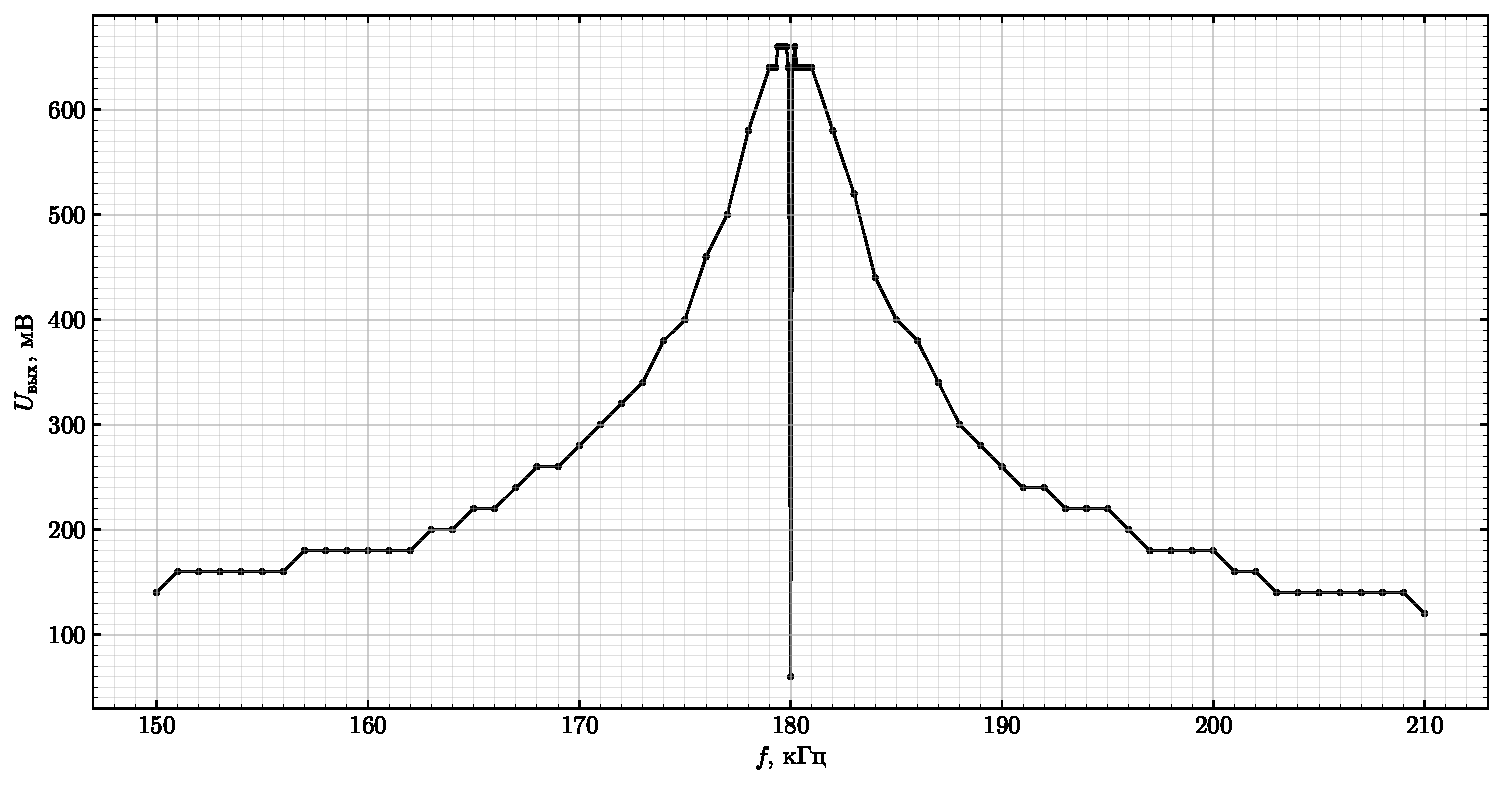
\includegraphics[width=\linewidth]{code/graph_1}
	\caption{АЧХ схемы при нагрузке $R_\text{н}$}
	\label{fig:pr:graph:1}
\end{figure}

Когда частота встроенного генератора совпадает с частотой подаваемого сигнала, огибающая содержит в себе только постоянную составляющую, при этом на осциллографе амплитуда наблюдаемого сигнала резко падает.

На графике $U_\text{вых}(f)$ наблюдается резкий спад амплитуды выходного сигнала на частоте
нулевых биений $f = 180~\text{кГц}$. Следовательно, это и есть частота встроенного генератора.

\subsection{Задание 2. Исследование нелинейности с резонансной нагрузкой}

Установили напряжение смещения $E_{\text{см}}=1{,}5~\text{В}$ и отключили шунтирующее сопротивление $R_{\text{ш}}$. На входы схемы подали сигналы амплитудой $1~\text{В}$: с первого канала генератора на разъём Вх1 сигнал частотой $180~\text{кГц}$, со второго канала на разъём Вх2 -- сигнал, частоту которого изменяли. Осциллограф подключили к разъёму КТ3. Снимали зависимость выходного напряжения от частоты одного генератора в двух диапазонах: от $1$ до $30~\text{кГц}$ и от $150$ до $200~\text{кГц}$ при неизменной частоте другого. В качестве нагрузки использовали $LC$-контур.

Полученная амплитудно-частотная характеристика приведена на рис. ниже:
\begin{figure}[H]
	\centering
	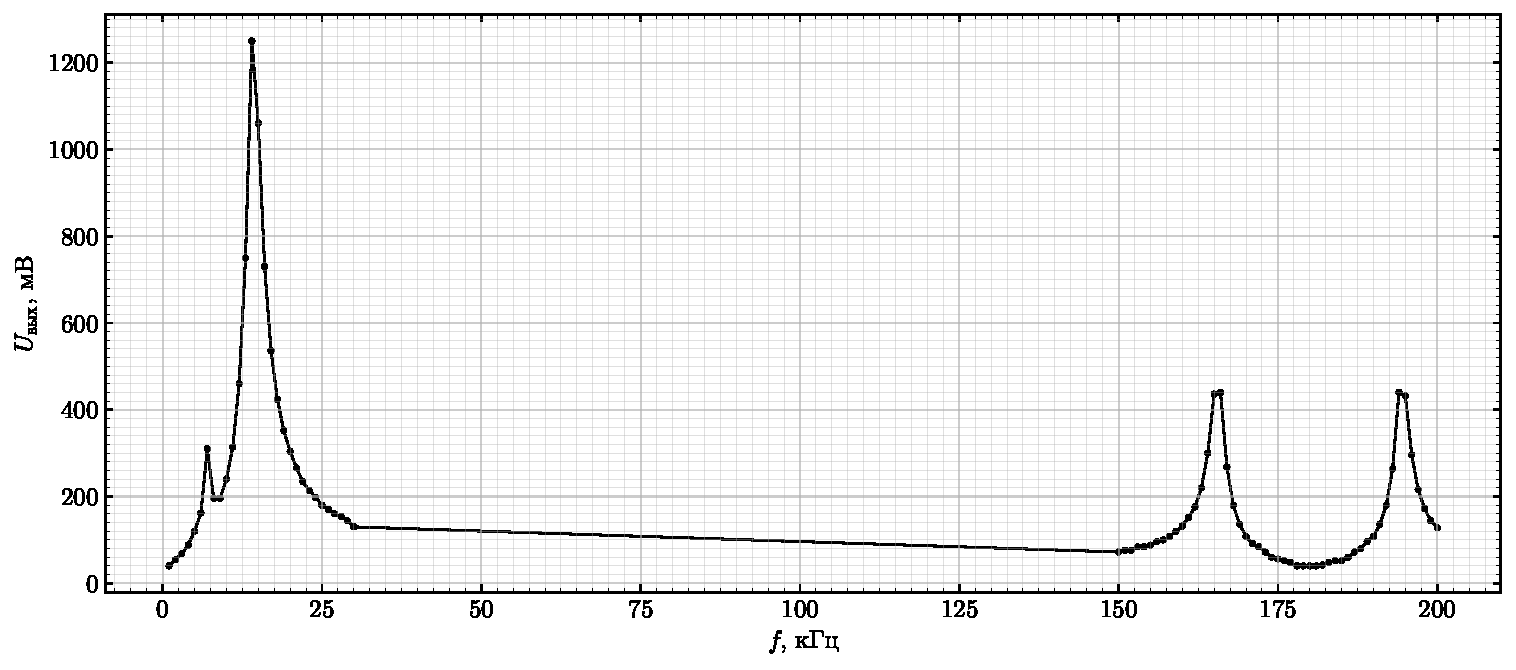
\includegraphics[width=1\linewidth]{code/graph_2}
	\caption{АЧХ преобразователя}
	\label{fig:pr:graph:2}
\end{figure}

В выходном сигнале нелинейной цепи должны присутствовать кратные и комбинационные частоты. Снятая зависимость представляет собой частотную характеристику преобразователя (зависимость модуля его комплексного коэффициента передачи от частоты принимаемого сигнала при постоянной частоте гетеродина). При взаимодействии колебаний некоторых частот сигнала с колебаниями частот $f_\text{г}$ и $n f_\text{г}$ получаются колебания промежуточной $f_\text{пч}$ частоты ($f_\text{рез} = f_\text{пч}$). Где $f_\text{рез}$ -- резонансная частота контура. Комбинационные частоты, совпадающие с $f_\text{пч}$ определяем в виде 
\[
m f_\text{г} - n f_s = f_\text{пч},~m f_s - n f_\text{г} = f_\text{пч}
\qquad\to\qquad
f_s = \frac{n}{m} f_\text{г} \pm \frac1m f_\text{пч}
\]

При $n=0$ и $m=1$ частота $f_s$ соответствует частоте прямого канала, т.е. $f_s = f_\text{пч}$.

При $n=1$ и $m=1$ преобразование осуществляется по первой гармонике частоты гетеродина:
\[
f_s = f \pm f_\text{пч}
\]

Мы определили резонансную частоту колебательного контура, а также комбинационные частоты:
\[
f_{\text{рез}} = f_{\text{пч}} = 14~\text{кГц}
\]
\[
f_{\text{г}} - f_{\text{пч}} = 166~\text{кГц}
\]
\[
f_{\text{г}} + f_{\text{пч}} = 194~\text{кГц}
\]

Отсюда частота генератора
\[
f_{\text{г}} = 180~\text{кГц},
\]

что близко к полученной ранее частоте генератора \(f_{\text{г}} = 180~\text{кГц}\).

\subsection{Задание 3. Исследование амплитудного детектора. Снятие детекторной характеристики}

В данном эксперименте включили вторую схему. Осциллограф подключили к разъёму КТ4; тумблером $T_2$ его можно переключать между входом генератора и выходом детектора.

Для снятия детекторной характеристики установили режим измерения постоянного напряжения (DC) и отключили нагрузочную ёмкость ($C=0$). На вход детектора через разъём КТ3 подали гармонический сигнал частотой $140~\text{кГц}$. Изменяя его амплитуду от $0{,}1$ до $2~\text{В}$, измеряли среднее выходное напряжение.

Полученная передаточная характеристика амплитудного детектора:
\begin{figure}[H]
	\centering
	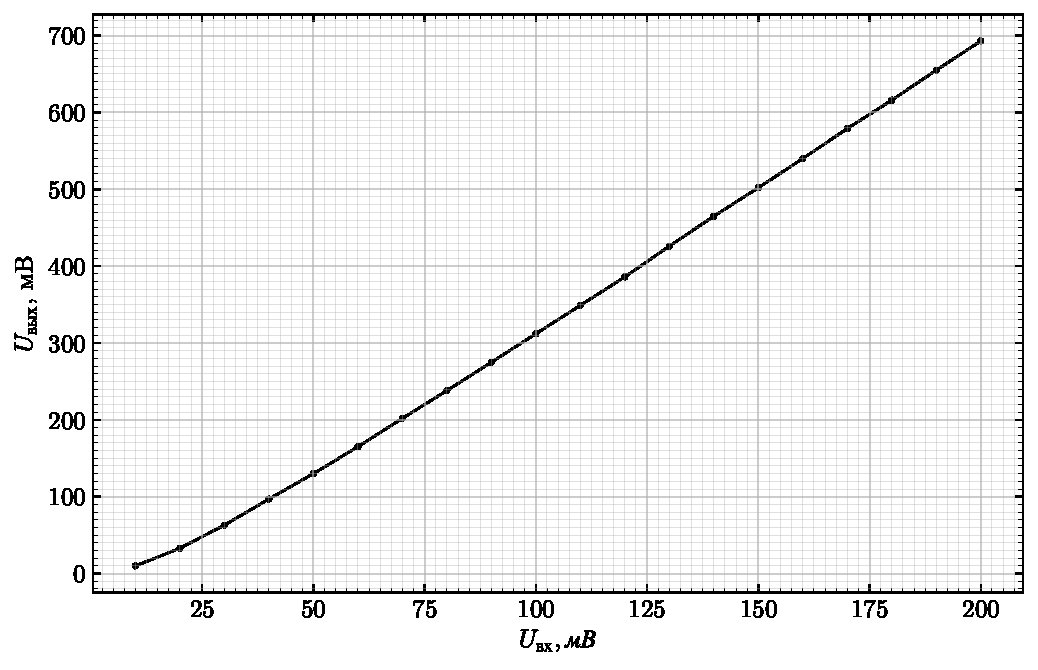
\includegraphics[width=\linewidth]{code/graph_3}
	\caption{Передаточная характеристика амплитудного детектора}
	\label{fig:pr:graph:3}
\end{figure}

На графике наблюдается увеличение среднего значения выходного напряжения при увеличении амплитуды входного сигнала. При амплитуде входного сигнала $U_{\text{вх}} = 1~\text{В}$ среднее значение выходного напряжения составляет $U_{\text{вых}} = 312~\text{мВ}$, а при амплитуде $U_{\text{вх}} = 2~\text{В}$ достигает $693~\text{мВ}$.

Коэффициент передачи детектора при амплитуде входного сигнала $1~\text{В}$ составляет:
\[
K_{\text{д}} = \frac{U_{\text{вых}}}{U_{\text{вх}}}
= \frac{0{,}312~\text{В}}{1~\text{В}} = 0{,}312
\]

Таким образом, передаточная характеристика амплитудного детектора является нелинейной. При увеличении амплитуды входного сигнала выходное напряжение возрастает, при этом характер зависимости изменяется в области малых амплитуд.

\subsection{Задание 4. Исследование зависимости выходного напряжения детектора от частоты модулирующего колебания при разных нагрузках}

Далее исследовали зависимость выходного напряжения от частоты модуляции при двух значениях ёмкости нагрузки: $C=0$ и $15~\text{нФ}$. Переключили осциллограф в режим измерения переменного напряжения (AC) и подали на вход детектора через разъём КТ3 амплитудно-модулированный сигнал с частотой несущей $140~\text{кГц}$ и глубиной модуляции $30\%$. Частоту модуляции изменяли от $1$ до $15~\text{кГц}$, измеряя амплитуду выходного сигнала. Осциллограммы входного и выходного сигналов для обоих значений ёмкости сохранены для отчёта.

Измеренные зависимости выходного напряжения:
\begin{figure}[H]
	\centering
	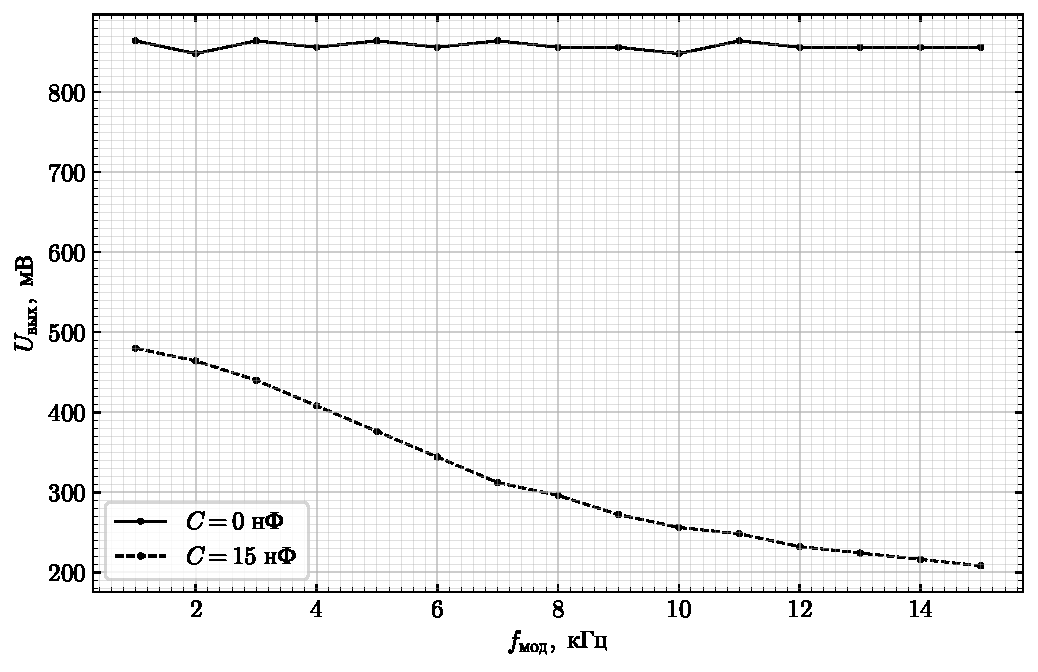
\includegraphics[width=\linewidth]{code/graph_4}
	\caption{Частотная характеристика амплитудного детектора при различных значениях емкости}
	\label{fig:pr:graph:4}
\end{figure}

При емкости $C = 0~\text{нФ}$ выходное напряжение практически не зависит от частоты и находится в диапазоне от $848$ до $864~\text{мВ}$.

При подключении конденсатора емкостью $C = 15~\text{нФ}$ наблюдается уменьшение выходного напряжения с ростом частоты. При частоте $f = 1~\text{кГц}$ напряжение составляет $480~\text{мВ}$, а при частоте $f = 15~\text{кГц}$ уменьшается до $208~\text{мВ}$.

Следовательно, емкость нагрузки оказывает существенное влияние на частотную характеристику детектора. При подключении конденсатора выходное напряжение уменьшается с увеличением частоты исследуемого сигнала.

\subsection{Задание 5. Резонансные характеристики при подключённом и отключённом детекторе}

В заключительном опыте исследовали резонансную характеристику при подключённом и отключённом детекторе. Установили ёмкость $3~\text{нФ}$, выход генератора подключили к разъёму КТ1, осциллограф -- к КТ4. Частоту входного сигнала изменяли в диапазоне от $5$ до $25~\text{кГц}$. Измерения провели сначала при разомкнутых разъёмах КТ3 и КТ4 (детектор отключён), затем при соединённых разъёмах (детектор подключён).

Полученные частотные характеристики:
\begin{figure}[H]
	\centering
	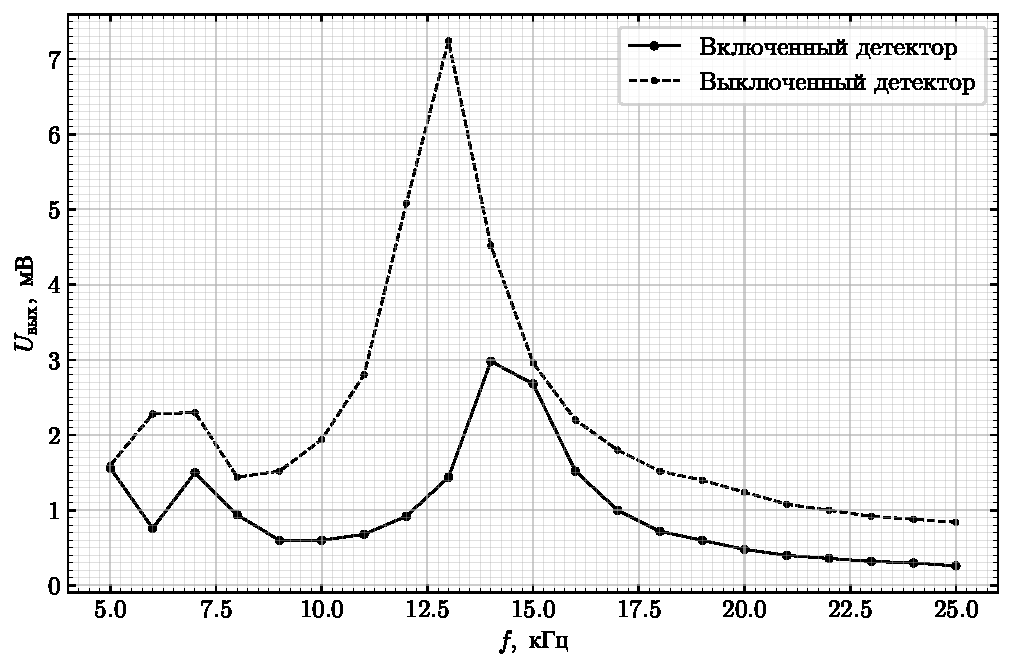
\includegraphics[width=\linewidth]{code/graph_5}
\caption{Резонансные характеристики при подключённом и отключённом детекторе}
	\label{fig:pr:graph:5}
\end{figure}

При подключённом детекторе максимум выходного напряжения наблюдается при частоте $f=14~\text{кГц}$ и достигает $2{,}98~\text{В}$. При дальнейшем увеличении частоты напряжение уменьшается и при $f=25~\text{кГц}$ составляет $0{,}26~\text{В}$.

При отключённом детекторе максимум выходного напряжения наблюдается при частоте $f=13~\text{кГц}$ и составляет $7{,}24~\text{В}$. При дальнейшем увеличении частоты напряжение уменьшается до $0{,}84~\text{В}$ при $f=25~\text{кГц}$.

Таким образом, подключение детектора уменьшает максимальное выходное напряжение и смещает частоту резонансного максимума с $13$ до $14~\text{кГц}$. Это показывает влияние входной нагрузки детектора на резонансную характеристику схемы.
